\section{Bayes' theorem}

Bayes' theorem describes the probability of an event to occur, depending on the prior knowledge of conditions related to the event \citep{bayesBasic}
\begin{equation}
\label{eqn:bayesianTheorem}
P(A|B) = \frac{P(B|A)P(A)}{P(B)},
\end{equation}
where P(A|B) is the posterior probability of A, given that B is true. P(B|A) is called conditional probability of B, given A being true. P(A) is the prior probability, the probability of A occurring without any additional information. Finally P(B) is the marginal probability of B, without any given condition. This theorem is often used for Bayesian inference, where it expresses how a belief, which is represented as probability, changes due to related evidence.	

\section{Bayesian inference}
\label{section:bayesianInference}

Bayesian inference is a process of data analysis to calculate the probability of a hypothesis depending on the available related evidence. As over time more and more evidence becomes available the probabilities can be updated, yielding a more sophisticated view on the hypothesis. It is given, according to Bayes' theorem, by
\begin{equation}
\label{eqn:bayesianInference}
P(H|E) = \frac{P(E|H)P(H)}{P(E)},
\end{equation}
where H represents a hypothesis and E some related evidence. P(H|E) is the posterior probability, which signifies the probability of the hypothesis after the evidence was observed. P(E|H) is called likelihood and it is the probability of observing the evidence, given the hypothesis. It is a measure of the compatibility of the observed evidence with the given hypothesis. P(H) is the prior probability, which is the probability of the hypothesis before any evidence is considered or obtained. P(E) is called marginal likelihood that represents the probability of the evidence being observed. However, it is independent of the chosen hypothesis. Thus, it is not factored in when comparing different hypotheses.
Bayesian inference can be applied to the "face in shadow" example of Section \ref{section:feedbackInVisualCortex}. There a neuron in V1 sees a small part of the visual field and signals if it sees an edge or not. At first it has the evidence of the observed pixels available and from it can calculate the likelihood that an edge is present. It has no prior knowledge of how probable an edge being present is, meaning that the prior probabilities for there being an edge or no edge are equal. With that likelihood and the prior probabilities it can conclude the posterior probability for the hypothesis "there is an edge" and decides that there is no edge.
Later, the inferior temporal cortex determines that there is a face in the picture and feeds this information back to V1. This influences the prior probabilities and changes the posterior probability. Through that, the V1 neuron starts to see the hypothesis  "there is an edge" as more likely, in order to complete the contour of the face. 
We now define X as a binary random vector of the visual input, Y as a multinomial variable of the output of V1 and Z as a multinomial variable of the feedback of the inferior temporal cortex. X is assumed independent of Z, when Y is given. This three node chain can be modelled as a generative probabilistic model and its visualization is given in Figure \ref{fig:generativeModel}. The figure shows the conditional dependence of Y on Z and of X on Y. In our case the prior is not constant as in Equation \ref{eqn:bayesianInference}, but it depends on Z. Thus, the prior is given by $P(Y|Z)$. The likelihood is given by $P(X|Y)$. When assuming different output classes K, we get the posterior $P(Y=k|X,Z)$ by plugging the likelihood and the prior into Equation \ref{eqn:bayesianInference}
\begin{equation}
\label{eqn:pYvorausgesetztXUndZ}
P(Y = k|X, Z) = \frac{P(X|Y=k)P(Y = k|Z)}{\Sigma_{k'}P(X|Y=k')P(Y=k'|Z)}.
\end{equation}

\begin{figure}
  \centering
  \label{fig:generativeModel}
  
\includegraphics[width=0.075\linewidth]{figures/generativeModel.png}
  \caption{Visual representation of the generative probabilistic model of the 3 node chain. It shows the interaction of the inferior temporal cortex, V1 and the visual input. It represents a multinomial mixture of 3 variables. X is a binary random vector of the visual input. Y is a multinomial variable of the output of V1 and Z is a multinomial variable of the feedback of the inferior temporal cortex. X is assumed independent of Z, when Y is given.}
\end{figure}

\section{Network model}

The network model used for the experiments in this thesis was taken from \citet{nessler} and expanded by an additional layer to include hierarchical feedback information.

\paragraph{Network architecture}
Rectangular images in black and white were given to the network. These images had varying sizes in the experiments, determined by their width $image_{width}$ and height $image_{height}$. Each pixel of an image was connected to two neurons. The first of these neurons is in an active state when the pixel is black and in an inactive state otherwise. The second neuron expresses the opposite behaviour. As a consequence the network needs $image_{width} \cdot image_{height} \cdot 2$ excitatory input neurons $x_1,...,x_N$. These input neurons are fully connected to the excitatory output neurons $y_1,...,y_K$. This means that every input neuron $x_i$ is connected to each output neuron $y_k$. 
To simulate the feedback from the inferior temporal cortex prior neurons, $z_1,...,z_J$, were added to the network. The prior neurons were also fully connected to the output neurons. The output neurons are modelled in a soft winner-takes-all (soft-WTA) circuit. The WTA behaviour was implemented via an adaptive inhibition signal $I(t)$. The adaptive inhibition is used to regulate the membrane potentials of the output neurons, so that all of them together fire with a total firing rate $R(t) = 200\text{ Hz}$ on average. A visualization of the network architecture can be seen in Figure \ref{fig:networkArchitecture}.

\begin{figure}
  \label{fig:networkArchitecture}
  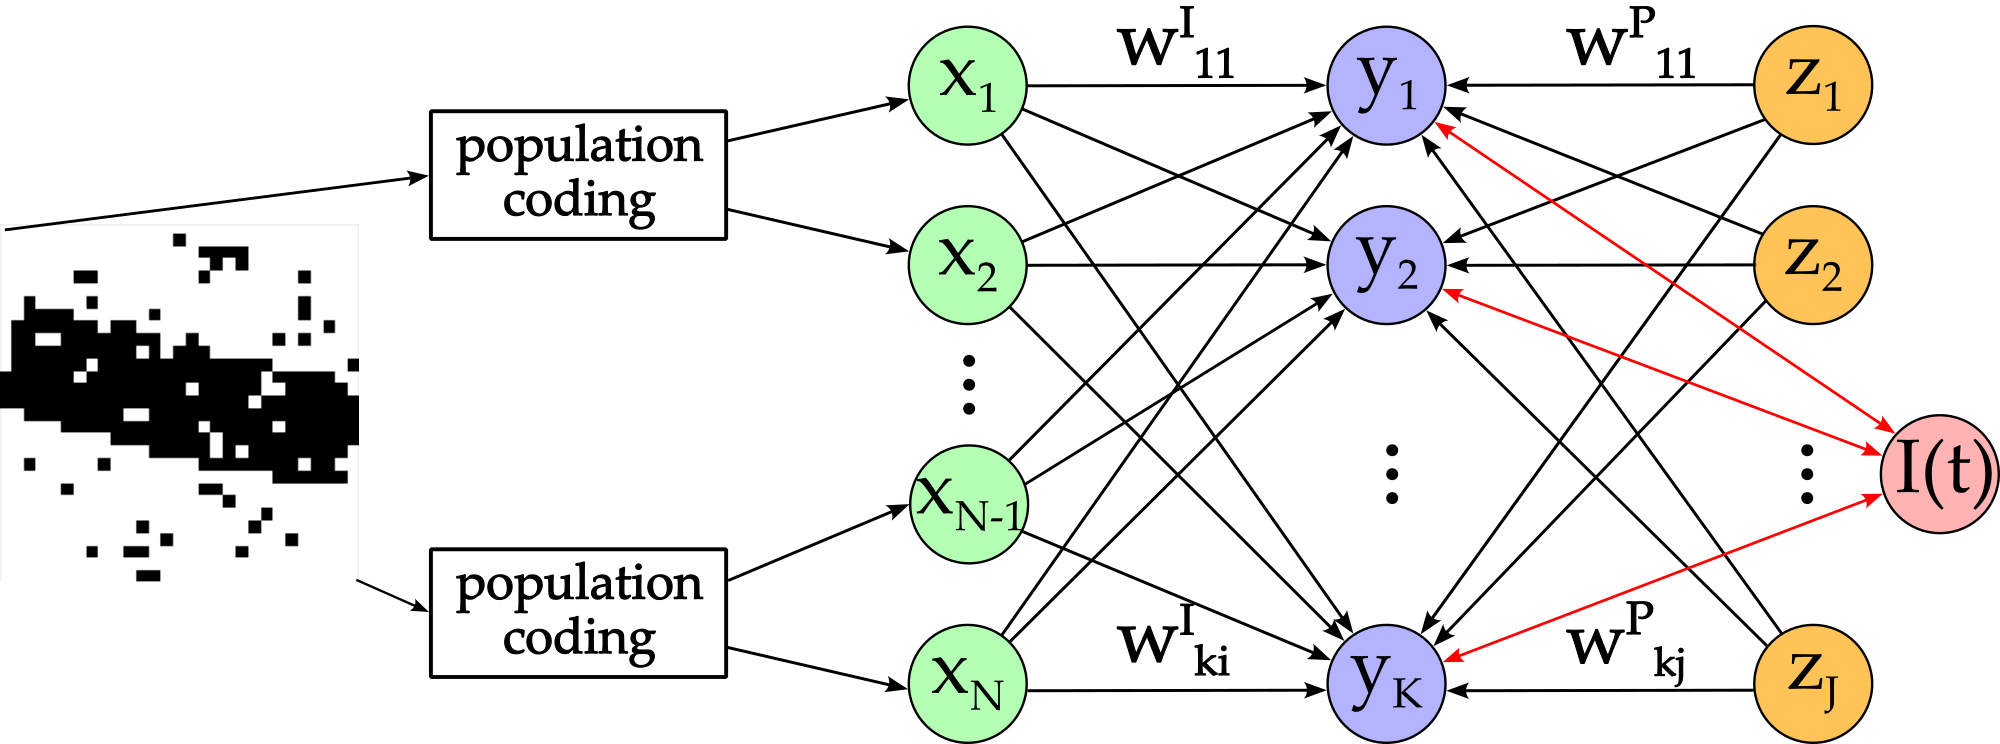
\includegraphics[width=\linewidth]{figures/networkPlan.png}
  \caption{Architecture of the network.}
\end{figure}

\paragraph{Neuron model}
As in \citet{nessler} the input neurons $x_1,...,x_N$ are firing according to a poisson process with an average firing rate $f_{input}$ when active and with 0 Hz when in an inactive state. The input neurons receive binary input, which is either a black, or a white pixel of an image. Each spike an input neuron generates was modelled by a double exponential kernel. As the signal is zero before the spike is generated, a Heaviside step function $\theta$ was applied to it, to limit the kernel to time ranges after the spike occurred. The Heaviside step function is given by
\begin{equation}
\theta (s) = \begin{dcases*} 1 & if $s \geq 0$ \\
0 & if $s < 0 $ \end{dcases*},
\end{equation}
where $s$ represents a time difference between the current simulation time and the time at which a spike occurred.
Multiplying $\theta(s)$ with the double exponential kernel yields the kernel function 
\begin{equation}
\varepsilon (s) = \theta (s) \cdot e^{-(s + \delta t) / \tau_{decay}} - e^{-(s + \delta t) / \tau_{rise}}.
\end{equation}
The kernel function has a time constant for the rise of the signal $\tau_{rise} = 1\text{ ms}$ and a time constant for the decay of the signal $\tau_{decay} = 15\text{ ms}$. The time step size of the simulation is $\delta t = 1\text{ ms}$. It had to be added to the double exponential kernel for numerical reasons, to evaluate the time at the end of the current simulation step, rather than at the beginning. A visualization of the kernel function can be seen in Figure \ref{fig:kernelFunction}. 

\begin{figure}
  \centering
  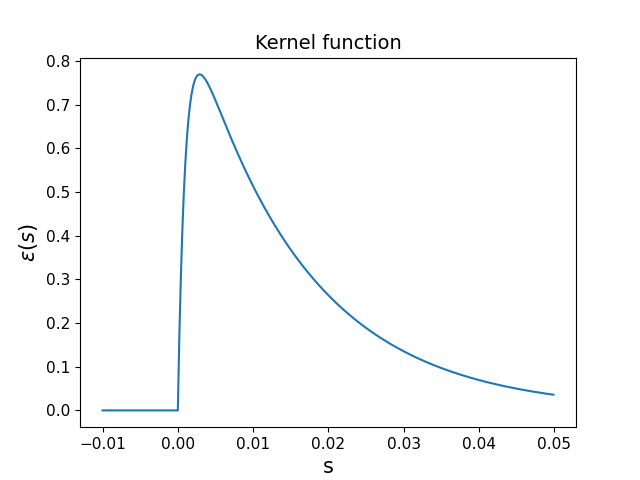
\includegraphics[width=0.6\linewidth]{figures/kernelFunction.png}
  \caption{Visualization of the kernel function $\varepsilon (s)$ within the relevant time window. A double exponential kernel was used. To limit the kernel function to positive values of s a Heaviside step function was applied. The output of this function was used to calculate the unweighed membrane potential response. }
  \label{fig:kernelFunction}
\end{figure}

Several input neuron spikes can happen in a short time window, increasing the unweighed membrane potential response $x_i(t)$. Depending on the timing of the spikes, they contribute additively to $x_i(t)$. The unweighed membrane potential response is given by

\begin{equation}
x_i(t) = \sum_{t_i^{(f)}} \varepsilon (t - t_i^{(f)}),
\end{equation}
with $t$ being the current simulation time and $t_i^{(f)}$ the time at which the input spike occurred.
Analogously, the unweighed membrane potential response of the prior neurons is given by
\begin{equation}
z_j(t) = \sum_{t_p^{(f)}} \varepsilon (t - t_p^{(f)}).
\end{equation}
 
The membrane potential $u_k$ of each output neuron is calculated by multiplying the unweighed membrane potential response of each input neuron times the input weight $w^{I}_{ki}$ of the connection between them, plus the unweighed membrane potential response of each prior neuron times the prior weight $w^{P}_{kj}$
\begin{equation}
\label{eqn:uk}
u_k(t) = \sum_{i=1}^N w^{I}_{ki} \cdot x_i(t) + \sum_{j=1}^J w^{P}_{kj} \cdot z_j(t).
\end{equation}
In \citet{nessler} each output neuron $y_k$ also had an intrinsic excitability $w_{k0}$, which was learned for each neuron. For the experiments of this thesis it was omitted, as the different classes of  input images were equally likely, thus the intrinsic excitabilities of the output neurons would all end up being equal to each other.

\citet{nessler} defined that the firing probability of an output neuron  $y_k$ is exponentially proportional to its membrane potential $u_k$ minus the received inhibition $I(t)$
\begin{equation}
\label{eqn:pVonY}
p(y_k \text{ fires at time t}) \propto e^{u_k(t) - I(t)}.
\end{equation}
This stochastic firing model is supported by experimental biological evidence \citep{woDasEHerkommt}. Through this definition the firing rate $r_k(t)$ of an output neuron is then modelled by an inhomogeneous Poisson process as
\begin{equation}
\label{eqn:rk}
r_k(t) = e^{u_k(t) - I(t)}.
\end{equation}
At every timestep of the simulation the inhibition signal $I(t)$ is subtracted from the membrane potential $u_k(t)$ of every output neuron. By that, the membrane potentials are altered to always yield a spiking frequency of 200 Hz, regardless if it would be lower or higher without it. This means that the adaptive inhibition signal can also function as an excitatory signal. 

The total firing rate of the output neurons $R(t)$	 is obtained by summing up the firing rates of all output neurons, yielding 
\begin{equation}
\label{eqn:R}
R(t) = \sum_{k=1}^K e^{u_k(t) - I(t)}.
\end{equation}

The inhibition signal $I(t)$ was chosen to depend on the current membrane potential of the output neurons. 
Solving Equation \ref{eqn:R} for $I(t)$ yields
\begin{equation}
\label{}
R(t) = \frac{ \sum_{k=1}^K e^{u_k(t)}}{e^{I(t)}}
\end{equation}
\begin{equation}
\label{}
e^{I(t)} = \frac{\sum_{k=1}^K e^{u_k(t)}}{R(t)}
\end{equation}
\begin{equation}
\label{}
I(t) = \ln{ \frac{ \sum_{k=1}^K e^{u_k(t)}}{R(t)}}
\end{equation}
\begin{equation}
\label{eqn:I(t)}
I(t) =  - \ln{R(t)} + \ln{  \sum_{k=1}^K e^{u_k(t)}}.
\end{equation}

The probability of an individual output neuron to fire within a time step $\delta t$ is given by
\begin{equation}
\label{eqn:rkdt}
r_k(t) \delta t.
\end{equation}

The conditional probability $q_k(t)$ that a spike originated from the output neuron $y_k$ is given by
\begin{equation}
\label{eqn:qk}
q_k(t) = \frac{r_k(t) \delta t}{R(t) \delta t} = \frac{e^{u_k(t) - I(t)}}{\sum_{k'=1}^K e^{u_{k'}(t) - I(t)}} = \frac{e^{u_k(t)}}{\sum_{k'=1}^K e^{u_{k'}(t)}}.
\end{equation}
The inhibition term cancels out because all output neurons receive the same inhibition, meaning that it is independent of k. Whenever an output spike should be generated within a time step, according to Equation \ref{eqn:rkdt}, it is determined via the discrete probability distribution $q_k(t)$ from which $y_k$ the spike originates. As $R(t)$ has a fixed value of 200 Hz, which is ensured by $I(t)$, it is unlikely that another output spike is generated shortly after the first one. This means, that the output spike generation functions as a soft-WTA function.
 
\paragraph{Spike timing dependent plasticity}
The input weights $w^{I}_{ki}$ between neurons $x_i$ and $y_k$ are updated whenever an output neuron fires. $\sigma$ determines the time window, after which spikes are no longer considered. If $y_k$ produces a spike, all its weights to the input neurons are updated as
\begin{equation}
\label{deltawki}
\Delta w^{I}_{ki} = \begin{dcases*} \lambda \cdot (ce^{-w^{I}_{ki}} - 1) & if $x_{i}$ fired in $ [t^f - \sigma, t^f] $ \\
\lambda \cdot (-1) & \text{if $ x_i $ did not fire in $ [t^f - \sigma, t^f] $, } \end{dcases*}
\end{equation}
where $\lambda$ is the learning rate, the hyperparameter c shifts the weight values, $t^f$ is the time when $y_k$ spiked and $\sigma$ is the time window in which input spikes are considered as "before" an output spike. As the membrane potentials $u_k$ of the output neurons result from the addition of the EPSPs of the input neurons times the corresponding weight, a way to control the average size of $u$ is needed. If $u$ is too small, the output neurons will fire too sparsely and if $u$ is too big, it will impair the learning process. So to limit $u$, the size of the weights is controlled via the hyperparameter c. The learning rate $\lambda$ is needed to control the size of each weight update. If it is too big, few output neurons will respond to too large parts of the input, while others might not respond at all. On the other hand if $\lambda$ is too small the network will learn very slowly and may never converge.
The prior weights $w^{P}_{kj}$ are also updated whenever an output neuron fires, in the same way as $w^{I}_{ki}$
\begin{equation}
\label{deltawkj}
\Delta w^{P}_{kj} = \begin{dcases*} \lambda \cdot (ce^{-w^{P}_{kj}} - 1) & if $z_{j}$ fired in $ [t^f - \sigma, t^f] $ \\
\lambda \cdot (-1) & \text{if $ z_j $ did not fire in $ [t^f - \sigma, t^f] $. } \end{dcases*}
\end{equation}

\section{Mathematical link between the spiking Winner-Take-All network model and Bayesian inference}
\label{linkNetworkBayes}

\citet{nessler} hypothesized that the ensemble of weights of a neuron can be understood as a generative model. They claimed that in a Bayesian inference context, every input spike provides evidence for an observed variable and every output spike represents one stochastic sample from the posterior distribution over hidden causes, which are encoded in the circuit. They further claimed, that every synaptic weight, due to STDP-induced changes,  converges stochastically to the log of the conditional probability that the presynaptic neuron has fired just before the postsynaptic neuron, given that the postsynaptic neuron fires. This connection is given by
\begin{equation}
\label{eqn:weightProbLink}
 w^{I}_{ki} = log(P(x_i = 1 | Y = k))
\end{equation}
and will be analysed in Section \ref{section:1D}.

The first model assumption is, that the Bayesian likelihood can be analytically calculated by
\begin{equation}
\label{eqn:P1}
P(X=\underline{x}|Y=k) = \prod_i P(x_i=1|Y=k)^{x_i} \cdot P(x_i=0|Y=k)^{(1-x_i)},
\end{equation}
where $\underline{x}$ is an encoded input vector. It has zeros where the input image has black pixels, and ones where there are white pixels. The conditional probability $P(x_i=1|Y=k)$ of an input pixel being white, given the output, is taken to the power of the probability that $x_i$ is active. This introduces a non-linear dependency on $x_i$. To capture the impact of black pixels, $P(x_i=0|Y=k)$ also has to be considered. It represents the conditional probability that a pixel is black, given the output. It is taken to the power of one minus the probability that $x_i$ is active, as the term should  be greatest, when $x_i = 0$.
$P(x_i=0|Y=k)$ can also be expressed as $1 - P(x_i=1|Y=k)$, as both together sum up to one. By utilizing this dependency and  expanding the equation by the natural logarithm we get
\begin{equation}
log P(X=\underline{x}|Y=k) = \sum_i (x_i log P(x_i=1|Y=k) + (1-x_i) log (1 - P(x_i=1|Y=k))).
\end{equation}
Utilizing Equation \ref{eqn:weightProbLink} and \ref{eqn:uk}  yields
\begin{equation}
log(P(X=\underline{x}|Y=k)) = \sum_i (x_i w^I_{ki} + (1-x_i)\overline{w^I_{ki}}) = u^X_k
\end{equation}
\begin{equation}
\Rightarrow P(X=\underline{x}|Y=k) = e^{u^X_k},
\end{equation}
where $u^X_k$ can be thought of as a partial membrane potential, caused by the activity of the input neurons.

According to the second model assumption, the Bayesian prior is given by
\begin{equation}
\label{eqn:P2}
P(Y=k|Z) = \prod_j P(Y=k|Z=j)^{z_j},
\end{equation}
where $P(Y=k|Z=j)$ is the conditional probability of the output neuron $y_k$ being active, given the prior neuron $z_j$ being active. $z_j$ equals one if that prior neuron is active, and zero if it is inactive. Rearranging the equation yields
\begin{equation}
log P(Y=k|Z) = \sum_j (z_j log P(Y=k|Z=j)).
\end{equation}
Utilizing Equation \ref{eqn:weightProbLink} and \ref{eqn:uk}  yields
\begin{equation}
log P(Y=k|Z) = \sum_j z_j w^P_{kj} = u^Z_k
\end{equation}
\begin{equation}
\Rightarrow P(Y=k|Z) = e^{u^Z_k},
\end{equation}
where $u^Z_k$ can be thought of as a partial membrane potential, caused by the activity of the prior neurons.

Inserting $P(X=\underline{x}|Y=k)$ and $P(Y=k|Z)$ into Equation \ref{eqn:pYvorausgesetztXUndZ} yields
\begin{equation}
\begin{split}
P(Y=k|X=\underline{x},Z) &= \frac{e^{u^X_k} e^{u^Z_k}}{\sum^K_{k'} e^{u^X_{k'}} e^{u^Z_{k'}}}\\
&= \frac{e^{u^X_k + u^Z_k}}{\sum^K_{k'} e^{u^X_{k'} + u^Z_{k'}}}\\
&= \frac{e^{u_k}}{\sum^K_{k'} e^{u_{k'}}}\\
&= q_k(t),
\end{split}
\end{equation}
which shows the connection between the Bayesian posterior and the conditional probability $q_k(t)$ of Equation \ref{eqn:qk}.
